% ============================================================
% Chapter 10 --- Learning the innovation law: EM for non-Gaussian chains
%
% Original work of this thesis. Builds directly on the grid-BP machinery
% of Chapter~\ref{ch:laplace} (\ref{sec:l-grid}), where the innovation law
% was assumed known. Here it is estimated. Numerical values are those of
% research/nongaussian-bp; full derivations and the complete experiment
% suite (27 experiments) are in that package's compendium and paper.
% ============================================================

\chapter{Learning the Innovation Law: EM for Non-Gaussian Chains}
\label{ch:em-method}

Chapters~\ref{ch:gaussian} and~\ref{ch:laplace} treated the transition law of
the clean chain as given: Gaussian in the first case, a fixed non-Gaussian
family in the second. Belief propagation then computed the diffusion score
exactly, in the Gaussian case, or against a validated numerical reference, in
the Laplace case. Neither chapter asked where the transition law itself comes
from. This chapter does. The clean data generating process is the same
first-order Markov chain of \eqref{eq:l-chain-prior}, but the innovation law
is now a member of an estimated family, and the question is how much the
Markov structure this thesis has exploited throughout still helps once part of
the model must be learned rather than assumed, and what breaks first when the
assumptions themselves are wrong.

\begin{quote}
How much does known Markov structure reduce the statistical and computational
burden of learning a diffusion score, and what is lost when the transition law
or the continuous messages must be approximated?
\end{quote}

The chapter answers the \emph{how} --- the estimator, what is exact in it and
what is numerical, and what the implementation was checked against.
Chapter~\ref{ch:em-results} answers the \emph{how much}.

\section{Model: an estimated mixture innovation}\label{sec:em-model}

The clean chain is, as in \eqref{eq:l-chain-prior},
\begin{equation}
  a_1 \sim \Nd(0,1), \qquad a_i = \alpha\, a_{i-1} + \varepsilon_i,
  \qquad i = 2,\dots,n,
  \label{eq:em-chain}
\end{equation}
with innovations $\varepsilon_i$ i.i.d., mean zero, variance
$q = 1-\alpha^2$, and now drawn from a member of a \emph{parametric family}
rather than a fixed law. Forward noising is the coordinatewise
Ornstein--Uhlenbeck channel of Section~\ref{sec:ou},
$x = e^{-t} a + \sqrt{\Deltat}\,\xi$, unchanged from every earlier chapter.

The estimated family is a $C$-component Gaussian mixture on the innovation,
\begin{equation}
  K_\theta(a' \mid a) = \sum_{c=1}^{C} \pi_c \,
    \Nd\!\big(a' - \alpha a;\ \nu_c,\ s_c^2\big),
  \qquad \theta = \{\alpha, (\pi_c,\nu_c,s_c)_{c=1}^C\},
  \label{eq:em-mixture-kernel}
\end{equation}
so both the autoregressive coefficient $\alpha$ and the shape of the
innovation density are free parameters, estimated jointly by maximum marginal
likelihood from noised data alone. At $C=1$ this collapses to a single
Gaussian, recovering the model of Chapter~\ref{ch:gaussian}; larger $C$ can
represent skew, heavy tails, and multimodality to the resolution of the
grid. The initial law $a_1 \sim \Nd(0,1)$ is \emph{held fixed} at
estimation time --- it is the value used to generate every family compared in
Chapter~\ref{ch:em-results}, so there is no misspecification in it, but
neither is there direct evidence it could itself be recovered from noised
data; that question is not addressed here.

Two assumptions are load-bearing and, consistent with the practice of this
thesis, are stated rather than tested by the estimator itself: the clean
process is exactly first-order Markov, and the forward noise is exactly
coordinatewise. Section~\ref{sec:em-nonmarkov} in the next chapter measures
what happens when the first of these is false by a controlled amount; the
second is never relaxed anywhere in this thesis.

\begin{remark}[Covariance-stationary, not strictly stationary]
Choosing $q=1-\alpha^2$ makes the chain covariance-stationary --- $\operatorname{Var}(a_i)=1$
and $\operatorname{Cov}(a_i,a_j)=\alpha^{|i-j|}$ hold exactly for \emph{every} innovation
law, by the same second-moment recursion as the Gaussian case. It does not
make the chain strictly stationary: for a non-Gaussian innovation the
invariant marginal law of the chain is not $\Nd(0,1)$, so fixing $a_1\sim
\Nd(0,1)$ starts every family off its own invariant distribution. Nothing
compared in this or the next chapter depends on the distinction, because every
family compared shares the same $a_1$ and the same covariance structure --- but
it is worth stating plainly, since an earlier draft of this material claimed
strict stationarity and that claim was too strong.
\end{remark}

\section{What remains exact}\label{sec:em-exact}

Two facts from Section~\ref{sec:l-grid} carry over unchanged and are worth
restating as the load-bearing structure of the whole estimator.

\begin{proposition}[The posterior factor graph is still the prior's chain]
\label{prop:em-unary}
Coordinatewise forward noising contributes exactly one \emph{unary} factor per
site, $x_i \mapsto \phi_i(a_i) \propto \exp\!\big(-(x_i-e^{-t}a_i)^2/2\Deltat\big)$.
It reweights node potentials and creates no new edges among the latent
$a_i$, for any innovation law, mixture or otherwise. The posterior over the
clean chain given the noised observation therefore factorises on exactly the
same chain graph as the prior.
\end{proposition}

\begin{proposition}[The E-step is exact]\label{prop:em-estep}
Since the posterior graph is a tree, one forward and one backward
sum-product sweep return the exact single-site and pairwise marginals of the
posterior, at the level of functional messages, for \emph{any} innovation
law. Consequently the E-step of an EM procedure for $\theta$ requires no
variational approximation and no sampling: the sufficient statistics EM needs
are exact conditional expectations under the true posterior, mixture label
included.
\end{proposition}

Both are consequences of the chain being a tree (Theorem~\ref{thm:tree-exact})
and hold independently of whether the innovation law admits a closed-form
message update. What is \emph{not} exact is the representation of a functional
message on a computer, which is where Section~\ref{sec:em-numerical} and the
grid-BP machinery of Section~\ref{sec:l-grid} enter.

\section{The EM algorithm}\label{sec:em-algorithm}

Write $\Xi(\theta)$ for the vector of exact posterior sufficient statistics
that BP supplies given the current parameter $\theta$ --- the conditional
expectations of the pairwise sums, mixture-label indicators, and second
moments that the mixture kernel's complete-data log-likelihood needs. The
gradient of the \emph{marginal} log-likelihood $\mathcal L(\theta)$ is given
by Fisher's identity,
\begin{equation}
  \nabla_\theta \mathcal L(\theta)
  = \big\langle \Xi(\theta),\ \nabla_\theta \log K_\theta \big\rangle .
  \label{eq:em-fisher}
\end{equation}
The practical content of \eqref{eq:em-fisher} is that belief propagation is
never differentiated through: BP supplies the conditional expectation
$\Xi(\theta)$ at the current parameter, and the gradient with respect to
$\theta$ is then an ordinary derivative of the kernel's log-density. This
is what makes the E-step of Proposition~\ref{prop:em-estep} directly usable
inside an optimiser.

The M-step for the mixture kernel is \emph{not} an exact maximisation. Given
$\Xi(\theta^{(k)})$, updating $(\pi_c,\nu_c,s_c)_{c=1}^C$ exactly would
require solving a mixture-likelihood problem with its own latent label, so the
implementation runs four inner conditional-maximisation sweeps instead --- the
algorithm is therefore generalised EM, or ECM \citep{meng1993maximum}, rather
than exact EM. Monotone ascent of $\mathcal L$ is guaranteed in theory by the
standard EM argument applied at the level of the surrogate $Q(\theta \mid
\theta^{(k)}) = \langle \Xi(\theta^{(k)}), \log K_\theta\rangle$, and was
checked directly: across an executable audit of the implementation, the
minimum increase in $Q$ over twelve consecutive steps was $+2.61$ for a
Gaussian kernel, $+4.34$ for Laplace, and $+4.18$ for an eight-component
mixture, with zero decreases recorded in every run logged by the project. One
correctness issue was found and fixed during that audit: two exit paths of
the fitting routine returned the kernel from one M-step \emph{before} the
last logged evidence value, so the reported convergence trace never covered
the model actually returned. The fix makes the returned kernel's evidence
equal to \texttt{trace.log\_evidence[-1]} by construction, with a regression
test asserting it.

\section{The numerical representation: grid BP, again}\label{sec:em-numerical}

Messages remain functions on $\R$, so they are represented exactly as in
Section~\ref{sec:l-grid}: values on $M$ equispaced points in $[-A,A]$, updates
by trapezoidal quadrature. Two error sources are tracked separately here as
well. Truncation error --- the probability mass the finite domain $[-A,A]$
misses --- is diagnosed by the worst boundary mass over the sites of a chain,
which falls from $3.4\times 10^{-4}$ at $A=4$ to $1.4\times10^{-8}$ at $A=8$
and does not depend on the grid resolution $M$. Quadrature error, from the
finite spacing $h=2A/M$ on an otherwise exact interior update, falls as
$O(h^2)$: a factor of four per halving of $h$, matching the trapezoidal
rate on a smooth integrand. At the working configuration used for every
experiment in this and the next chapter, $M=401$, $A=8$, both sources sit far
below any effect subsequently measured: the discretised recursion reproduces
the closed-form Gaussian posterior mean to $9.2\times10^{-15}$, and agrees
with an independently coded brute-force enumeration --- sharing no code with
the BP recursion --- to $1.6\times10^{-14}$ on posterior means and
$1.8\times10^{-15}$ on the log-evidence.

\begin{figure}[t]\centering
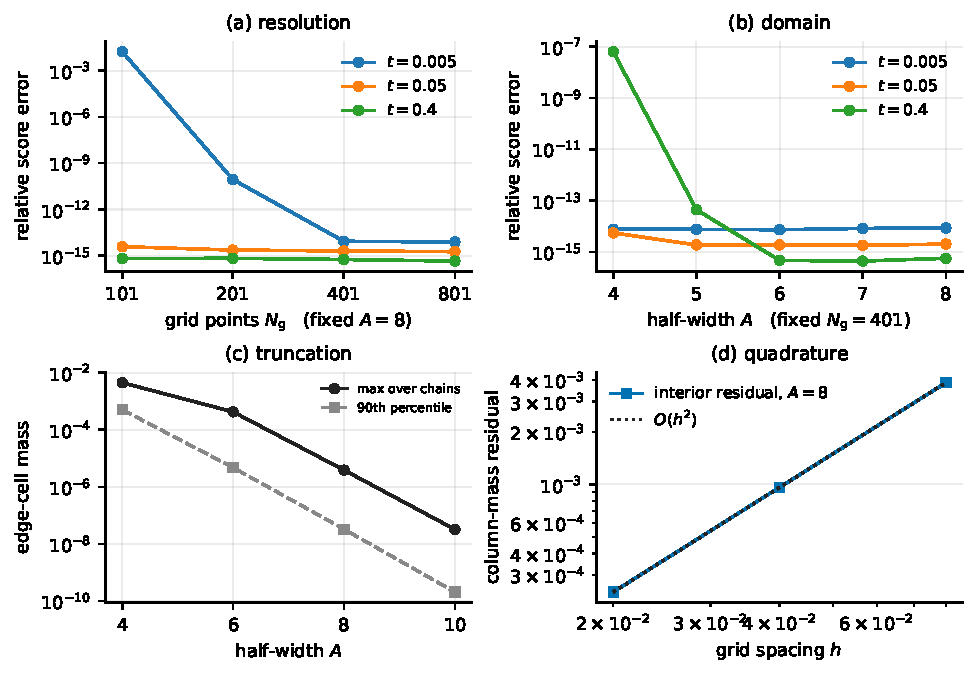
\includegraphics[width=0.72\linewidth]{figures/fig_grid_domain.pdf}
\caption{Grid and domain control on a Laplace chain ($\alpha=0.85$, $n=32$
sites). Left: relative score error against a high-resolution reference as
grid resolution $M$ grows at fixed half-width $A=8$. Right: the same as the
domain half-width $A$ grows at fixed $M=401$. Both saturate at the
floating-point floor well inside the working configuration. Source:
\texttt{outputs/exp\_02\_grid\_convergence/}.}
\label{fig:em-grid-domain}
\end{figure}

\begin{remark}[The boundary-mass diagnostic is empirical, not a bound]
\label{rmk:em-boundary}
The worst-boundary-mass figures above were originally computed from a single
sampled chain and reported as if they bounded the truncation error for every
run. They do not: reseeding the same diagnostic over 256 independent chains
per configuration shows the single-chain value sits near the \emph{median}
over chains, while the maximum observed is up to $152\times$ higher (range
$2.9\times$ to $8369\times$ across configurations). The diagnostic should be
read as an empirical estimate of typical truncation loss, not a certified
bound. What it does \emph{not} affect is the separation of truncation from
quadrature error reported above, which is a pure function of $(A,M)$ and the
prior and involves no sampled chain at all --- that comparison reproduces
to $0.000$ relative difference under reseeding and is exactly the result
Section~\ref{sec:l-grid} already relies on.
\end{remark}

One further identity is worth restating from Section~\ref{sec:l-grid} because
it governs every result in the next chapter exactly as it governed
Chapter~\ref{ch:laplace}: whatever an approximation --- Gaussian closure, grid
truncation, or an under-converged fit --- does to the posterior mean is
amplified by $e^{-t}/\Deltat \sim 1/2t$ in the score, so small diffusion times
remain the regime where any deficiency is most visible.

\begin{figure}[t]\centering
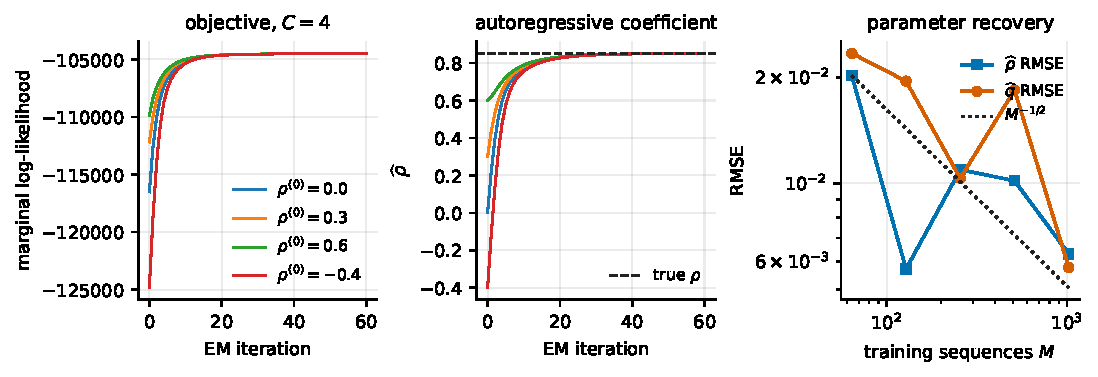
\includegraphics[width=0.9\linewidth]{figures/fig_em_diagnostics.pdf}
\caption{Optimisation diagnostics for the EM procedure of
Section~\ref{sec:em-algorithm}. Left: marginal log-likelihood by iteration
from four initialisations of $\alpha$; the largest decrease across
iterations is zero in every run. Centre: the estimated $\alpha$ over the
same runs, converging to $[0.8517,0.8520]$ against a truth of $0.85$ from
initialisations spanning $[-0.4,0.6]$ --- direct evidence that $\alpha$ is
estimated, not supplied. Right: RMSE of the recovered $\alpha$ and
innovation variance against the number of training sequences, with an
$n^{-1/2}$ reference line. Source: \texttt{outputs/exp\_18/} and
\texttt{outputs/exp\_06\_em\_parameter\_recovery/}.}
\label{fig:em-diagnostics}
\end{figure}

\section{What convergence actually costs}\label{sec:em-convergence}

The last piece of machinery this chapter reports is not a theorem but a
measurement, and it is the one that most directly qualifies the results of
Chapter~\ref{ch:em-results}: how many EM iterations the algorithm of
Section~\ref{sec:em-algorithm} actually needs.

Two arms of the same chains were fit under identical initialisation and
budget, one seeing clean data and the other once through the OU channel:

\begin{center}
\begin{tabular}{@{}rcccc@{}}
\toprule
iteration & \multicolumn{2}{c}{clean} & \multicolumn{2}{c}{through the channel} \\
 & $\alpha$ & kurtosis & $\alpha$ & kurtosis \\
\midrule
1   & 0.8473 & 1.470 & 0.4276 & 0.112 \\
30  & 0.8467 & 2.858 & 0.8366 & 1.527 \\
120 & 0.8473 & 3.014 & 0.8464 & 3.164 \\
600 & 0.8475 & 3.132 & 0.8466 & 3.096 \\
\bottomrule
\end{tabular}
\end{center}
\noindent(truth: $\alpha=0.85$, innovation kurtosis $3.0$). Both arms reach
the truth; what differs is the \emph{rate}. On clean data $\alpha$ is
converged after a single M-step, since nothing about it is hidden at the
chain level. Through the channel it takes on the order of $30$--$60$
iterations --- the missing-information mechanism of
\citet{dempster1977maximum} appearing directly in the convergence rate, where
the theory places it. The innovation shape is slower still, and on \emph{clean}
data already: tens of iterations against one for $\alpha$, because the
mixture label is itself a latent variable even without an observation
channel. The channel then compounds this. A dedicated sweep measuring exactly
how many iterations the slowest configuration needs found roughly
\textbf{2000} --- about $50\times$ a budget of 40 iterations, which several of
the experiments reported in Chapter~\ref{ch:em-results} used as a fixed
default before this measurement existed.

\begin{remark}[Fixed budgets compare convergence rates, not estimators]
\label{rmk:em-fixed-budget}
This is the single methodological lesson of the chapter, and it recurs
throughout the next one. Whatever coordinate of a fit converges slower looks
worse under a fixed iteration count, and a slower-converging configuration
under-iterated by the same budget produces what looks like a genuine deficit
rather than symmetric noise --- which is precisely the signature that makes it
easy to mistake for a real effect. An eight-seed replication at the same
fixed budget of 200 iterations found no channel penalty on converged shape
recovery once compared correctly (paired clean $-$ noised difference
$-0.052\pm0.217$, consistent with zero) --- retiring an earlier claim that
had rested on a single non-converged draw. Where Chapter~\ref{ch:em-results}
reports a result obtained at a fixed, possibly insufficient budget, it says so
explicitly and states which quantities are and are not affected.
\end{remark}

\section{Summary}

The estimator combines two facts that hold for any innovation law ---
Proposition~\ref{prop:em-unary} and Proposition~\ref{prop:em-estep} --- with a
generalised M-step and Fisher's identity to turn exact BP conditional
expectations into a marginal-likelihood gradient. Everything about the
\emph{posterior inference} step is exact up to the grid discretisation of
Section~\ref{sec:em-numerical}, which is controlled to far below any effect
measured. What is not free is optimisation time: the innovation shape is an
order of magnitude slower to converge than the autoregressive coefficient,
and by a further order of magnitude once observed only through noise.
Chapter~\ref{ch:em-results} reports what this estimator buys --- in data
efficiency and, separately, in the fidelity of what it generates --- and where,
along axes of model capacity and model misspecification, it stops buying
anything.
